%%%%%%%%%%%%%%%%%%%%%%%%%%%%%%%%%%%%%%%%%%%%%%%%%%%%%%%%%%%%%%%
%
% Welcome to Overleaf --- just edit your LaTeX on the left,
% and we'll compile it for you on the right. If you open the
% 'Share' menu, you can invite other users to edit at the same
% time. See www.overleaf.com/learn for more info. Enjoy!
%
%%%%%%%%%%%%%%%%%%%%%%%%%%%%%%%%%%%%%%%%%%%%%%%%%%%%%%%%%%%%%%%
\documentclass{article}
\usepackage{minted}
\usepackage{lipsum,graphicx}
\usepackage{amsmath}
\usepackage{xcolor} % to access the named colour LightGray
\definecolor{LightGray}{gray}{0.9}

\title{Report 2 \\ \textsc{Modeling of Continuous Systems}} % Title

\author{Fernando Gabriel\\ % Author name\\
Student ID: 22M12329}

\date{\today} % Date for the report

\begin{document}

\maketitle % Insert the title, author and date


\section{Problem 1}
\subsection*{Code}
\begin{minted}
[
frame=lines,
framesep=2mm,
baselinestretch=1.2,
bgcolor=LightGray,
fontsize=\footnotesize,
linenos
]
{matlab}
clc, clear all;
%% Set symbolic variables
syms f real % input

syms x th real % outputs
syms dx dth real % first derivatives
syms ddx ddth real % second derivatives

syms M m g l real % systems constants

%% Define the system
% States of systme
q = [x; th];
dq = [dx; dth];
ddq = [ddx; ddth];

q_dq = [q; dq];
dq_ddq = [dq; ddq];

% Postion of mass M
x_M = [x, 0];
% Postion of mass m
x_m = [x + sin(th) * l, cos(th) * l];

%% Velocity of each element of the system
dx_Mdt = jacobian(x_M, q) * dq;
dx_mdt = jacobian(x_m, q) * dq;

%% Kynetic Energy of the system
% Sum of both kynectic energies
K = 1/2 * M * (dx_Mdt' * dx_Mdt) + 1/2 * m * (dx_mdt' * dx_mdt);

%% Potential Energy with respect th = 0
U = g * M * x_M(2) + g * m * x_m(2);

%% Lagangian
L = K - U;

% Lagrangian calculation, equation without imputs
eq = jacobian(jacobian(L, dq), q_dq) * dq_ddq - jacobian(L, q)';
eq = simplify(eq);

% Get matrix A
A = jacobian(eq, ddq);
% Get constants
B = simplify(eq - A * ddq);

%% Assemble system in matrix form with inputs
Eq_left = A * ddq;
Eq_right = [f; 0] - B;

Eq = Eq_left == Eq_right;
pretty(Eq)

%% Getting the solution by using the inverse matrix
sol_ddq = simplify(A \ Eq_right);
pretty(sol_ddq)

%% Equilibrium conditions
eq_q = [0; 0];
eq_dq = [0; 0];
eq_f = 0;

%% Linearization
linearized_eq = subs(jacobian(sol_ddq, q), [q_dq; f], [eq_q; eq_dq; eq_f]) * dq + ...
subs(jacobian(sol_ddq, f), [q_dq; f], [eq_q; eq_dq; eq_f]) * f;

\end{minted}
\subsection*{Results}
Non linear systems after applying Lagrangian
\begin{equation}
   \left(\begin{array}{c} \ddot{x}\,\left(M+m\right)+\ddot{\theta}\,l\,m\,\cos\left(\theta\right)=l\,m\,\sin\left(\theta\right)\,{\dot{\theta}}^2+f\\ \ddot{\theta}\,m\,l^2+\ddot{x}\,m\,\cos\left(\theta\right)\,l=g\,l\,m\,\sin\left(\theta\right) \end{array}\right)
\end{equation}
Matrix A and B are:
\begin{equation*}
   A = \left(\begin{array}{cc} M+m & l\,m\,\cos\left(\theta\right)\\ l\,m\,\cos\left(\theta\right) & l^2\,m \end{array}\right)
\end{equation*}

\begin{equation*}
   B = \left(\begin{array}{c} -{\dot{\theta}}^2\,l\,m\,\sin\left(\theta\right)\\ -g\,l\,m\,\sin\left(\theta\right) \end{array}\right)
\end{equation*}
We use them to get the matrix form of the system.\\
Solution of the system is:
\begin{equation*}
   \left(\begin{array}{c} \ddot{x}\\ \ddot{\theta} \end{array}\right) =\left(\begin{array}{c} \frac{l\,m\,\sin\left(\theta\right)\,{\dot{\theta}}^2+f-g\,m\,\cos\left(\theta\right)\,\sin\left(\theta\right)}{-m\,{\cos\left(\theta\right)}^2+M+m}\\ -\frac{l\,m\,\cos\left(\theta\right)\,\sin\left(\theta\right)\,{\dot{\theta}}^2+f\,\cos\left(\theta\right)-g\,m\,\sin\left(\theta\right)-M\,g\,\sin\left(\theta\right)}{l\,\left(-m\,{\cos\left(\theta\right)}^2+M+m\right)} \end{array}\right)
\end{equation*}
Linearized system for equilibrium conditions $x_0 = 0 \, \theta_0 = 0 $
\begin{equation*}
   \left(\begin{array}{c} \Delta{\ddot{x}}\\ \Delta{\ddot{\theta}} \end{array}\right)  = \left(\begin{array}{c} \frac{f}{M}-\frac{\Delta{\theta}\,g\,m}{M}\\ \frac{\Delta{\theta}\,\left(M\,g+g\,m\right)}{M\,l}-\frac{f}{M\,l} \end{array}\right)
\end{equation*}

To verify the derivation for the state equation of the
inverted pendulum, we followed the following steps:
\begin{enumerate}
   \item Define the position of the mass M and m
   \item Calculate the velocity of each mass
   \item Calculate the total kinetic energy of the system
   \item Calculate the potential energy of the system
   \item Get the Lagangian based on the kinetic and potential energy
   \item Apply Lagrange's equations to get the differential equations of the system
   \item Transforming it into state space equation
   \item Solve the values of the second time derivative of the states of the system, $\ddot{x}\, \ddot{\theta}$
\end{enumerate}
To do most of the above steps, we used symbolic variable and the build in function \textbf{jacobian}.
\newpage
\section{Problem 2}


\begin{minted}
   [
   frame=lines,
   framesep=2mm,
   baselinestretch=1.2,
   fontsize=\footnotesize,
   linenos
   ]
   {matlab}
   clc, clear all, close all;
   M = [0, 1, 2, 10];

   % Range of x
   x = -pi:0.1:pi;
   figure()
   % Plot original curve
   plot(x, sin(x), '-x','LineWidth', 2);
   hold on
   grid on
   
   % Plot expanded curves for different values of m
   for i = 1:length(M)
       m = M(i);
       plot(x, mySine(x, m), 'LineWidth', 2)
   end
   
   legend('sin', 'm=0', 'm=1', 'm=2', 'm=10')
   
   title('Sine function expansion');
   
   %% Function to calculate the expanded sine function
   function fx = mySine(x, m)
       fx = 0;
   
       for k = 0:m
           fx = fx + (-1)^k * myFactorial(2 * k +1) * x.^(2 * k + 1);
       end
   
   end
   %% Function to calculate the inverse factorial
   function x = myFactorial(k)
       x = 1 / factorial(k);
   end
   % function X = myFactorial2(k)
   %  X = 1;

   %  for i = 1:k
   %      X = X * i;
   %  end

   %  X = 1 / X;

   % end
   \end{minted}


\begin{figure}[H]
   \centering
   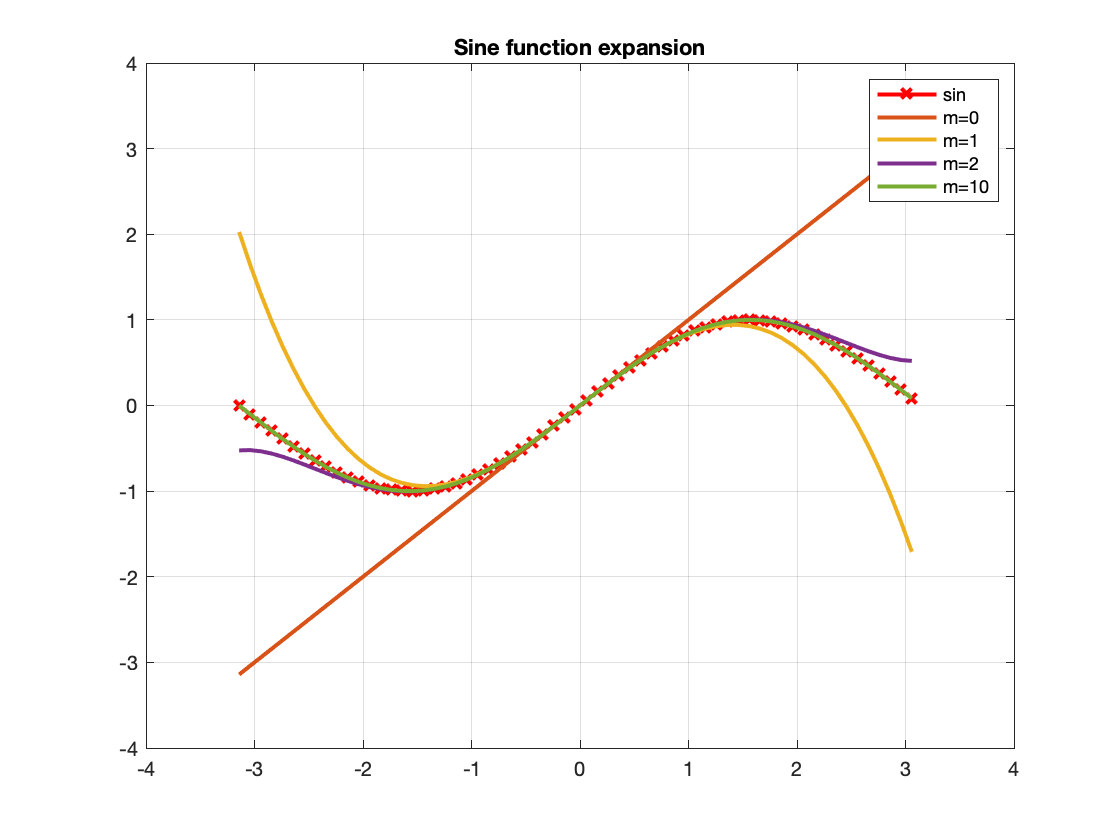
\includegraphics[width=.8\columnwidth]
   {imgs/sin_expansion.png}
   \caption{Comparison of plot for different m}
\end{figure}
We can observe a tendency to get closer to the real curve when using more expansion terms
\end{document}